\documentclass[tikz,border=5pt]{standalone}
\usepackage[T1]{fontenc}
\usepackage{helvet}
\renewcommand{\familydefault}{\sfdefault}
\usetikzlibrary{arrows.meta}
\definecolor{ink}{HTML}{202020}
\definecolor{skill}{HTML}{496A92}
\definecolor{memory}{HTML}{377C70}
\definecolor{reflectorbg}{HTML}{F3F3F3}
\definecolor{optimizerbg}{HTML}{E9E9E9}
\begin{document}
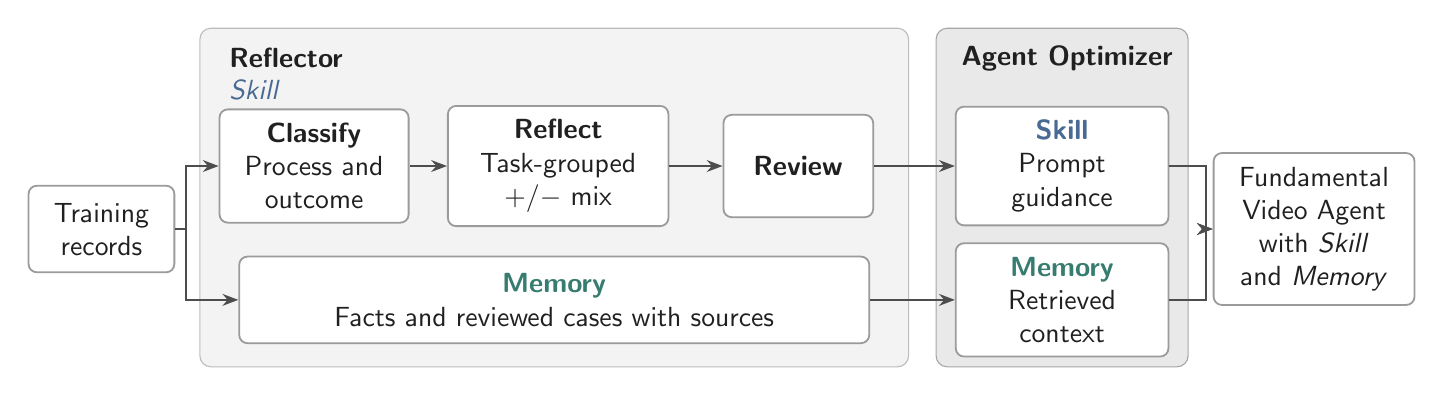
\begin{tikzpicture}[
    x=1cm,y=-1cm,
    every node/.style={font=\sffamily\fontsize{10}{12}\selectfont,text=ink},
    box/.style={draw=ink!45,fill=white,rounded corners=3pt,
        line width=.65pt,align=center,inner sep=5pt,minimum height=1.1cm},
    skillbox/.style={box},
    memorybox/.style={box},
    flow/.style={-{Stealth[length=2mm]},line width=.8pt,draw=ink!80}
]
\filldraw[fill=reflectorbg,draw=ink!30,rounded corners=4pt]
    (2.2,.1) rectangle (11.2,4.4);
\filldraw[fill=optimizerbg,draw=ink!40,rounded corners=4pt]
    (11.55,.1) rectangle (14.75,4.4);
\node[anchor=west,font=\sffamily\bfseries] at (2.45,.48) {Reflector};
\node[anchor=west,font=\sffamily\bfseries] at (11.75,.48) {Agent Optimizer};
\node[anchor=west,text=skill] at (2.45,.88) {\textit{Skill}};

\node[box,text width=1.5cm] (input) at (.95,2.65)
    {Training\\records};
\node[skillbox,text width=2.05cm,minimum height=1.3cm] (classify) at (3.65,1.85)
    {\textbf{Classify}\\Process and outcome};
\node[skillbox,text width=2.45cm,minimum height=1.3cm] (reflect) at (6.75,1.85)
    {\textbf{Reflect}\\Task-grouped\\$+/-$ mix};
\node[skillbox,text width=1.55cm,minimum height=1.3cm] (review) at (9.8,1.85)
    {\textbf{Review}};
\node[memorybox,text width=7.65cm] (memory) at (6.7,3.55)
    {\textbf{\textcolor{memory}{\textit{Memory}}}\\Facts and reviewed cases with sources};

\draw[flow] (input.east) -- (2.02,2.65) |- (classify.west);
\draw[flow] (input.east) -- (2.02,2.65) |- (memory.west);
\draw[flow] (classify) -- (reflect);
\draw[flow] (reflect) -- (review);

\node[skillbox,text width=2.35cm,minimum height=1.3cm] (loadskill) at (13.15,1.85)
    {\textbf{\textcolor{skill}{\textit{Skill}}}\\Prompt guidance};
\node[memorybox,text width=2.35cm] (loadmemory) at (13.15,3.55)
    {\textbf{\textcolor{memory}{\textit{Memory}}}\\Retrieved context};
\draw[flow] (review) -- (loadskill);
\draw[flow] (memory) -- (loadmemory);

\node[box,text width=2.2cm,minimum height=1.75cm] (agent) at (16.35,2.65)
    {Fundamental\\Video Agent\\with \textit{Skill}\\and \textit{Memory}};
\draw[flow] (loadskill.east) -- (14.98,1.85) |- (agent.west);
\draw[flow] (loadmemory.east) -- (14.98,3.55) |- (agent.west);
\end{tikzpicture}
\end{document}
